% =====================================================================
%  LaTeX Workshop: your working file
% =====================================================================
%  Everything after a % on a line is a comment: LaTeX ignores it.
%
%  Work through the TODOs block by block.
%  Search for "TODO 2." to find every TODO of block 2.
%  Some TODOs have parts in more than one place, e.g. in the preamble.
%
%  The text of the report is already here, as comments.
%  Write your own, or uncomment it: select the lines and press Ctrl+/
%  (Cmd+/ on a Mac).
%  The TODOs are about the commands around the text.
%
%  Stuck? Copy checkpoints/checkpoint-0n.tex over this file
%  (n is the block that just ended) and continue from there.
% =====================================================================

% TODO 1.1: Compiling document
<<<
@0
%   Write Hello OST! on the line after \begin{document}, then compile.
@1
>>>
\documentclass[a4paper, 11pt]{article}

% TODO 2.6: Paragraph spacing
<<<
@0
%   Load the parskip package here.
@2
\usepackage{parskip}
>>>

% TODO 3.3: Derivation
<<<
@0
%   Load the amsmath package here.
@3
\usepackage{amsmath}
>>>

% TODO 4.1: Table with booktabs
<<<
@0
%   Load the caption and booktabs packages here.
@4
\usepackage{caption}
\usepackage{booktabs}
>>>

% TODO 4.2: Figure
<<<
@0
%   Load the graphicx package here.
@4
\usepackage{graphicx}
>>>

% TODO 4.5: Citation
<<<
@0
%   Load biblatex and add the bibliography file here:
%       \usepackage[backend=biber, style=numeric]{biblatex}
%       \addbibresource{references.bib}
@4
\usepackage[backend=biber, style=numeric]{biblatex}
\addbibresource{references.bib}
>>>

% TODO 4.4: Clickable references
<<<
@0
%   Load the hyperref package here, as the last package.
%   Then add \hypersetup{hidelinks}, so links get no coloured boxes.
@4
\usepackage{hyperref}
\hypersetup{hidelinks}
>>>

% TODO 2.7: Bold emphasis (optional)
%   Add this line here and compile:
%       \renewcommand{\emph}[1]{\textbf{#1}}

% TODO 1.2: Title block
<<<
@0
%   Add \title, \author and \date here, and \maketitle further down.
%       Title:  How Fast Does Your Coffee Go Cold?
%       Author: your name
%       Date:   \today
@1
\title{How Fast Does Your Coffee Go Cold?}
\author{Your Name}
\date{\today}
>>>

\begin{document}

% TODO 1.2: Title block
<<<
@0
%   \maketitle goes here.
@1
\maketitle
>>>

% TODO 1.4: Table of contents
<<<
@0
%   Add \tableofcontents here and compile.
@1
\tableofcontents
>>>

% TODO 1.3: Sections
<<<
@0
%   Replace Hello OST! with the five sections, each at its own TODO 1.3:
%   Introduction, Theory, Setup, Results, Conclusion.
%   Then uncomment the Introduction text below, or write your own.
%   \section{Introduction} goes here.
@1
\section{Introduction}
@4
\section{Introduction}\label{sec:introduction}
>>>

% TODO 1.5: Styled words
<<<
@0
%   In the text below, set Newton's law of cooling in italics (\textit),
%   everyday vessels in bold (\textbf) and mug, glass and flask in
%   typewriter (\texttt).
% A freshly poured coffee is too hot to drink, and a forgotten one is too cold.
% Somewhere in between there is a window of a few minutes in which the drink is actually pleasant,
% and this report sets out to find it.
% The underlying physics is Newton's law of cooling,
% which says that a body loses heat in proportion to how much hotter it is than its surroundings.
% Three everyday vessels are compared,
% referred to throughout by the short labels mug, glass and flask.
@1
A freshly poured coffee is too hot to drink, and a forgotten one is too cold.
Somewhere in between there is a window of a few minutes in which the drink is actually pleasant,
and this report sets out to find it.
The underlying physics is \textit{Newton's law of cooling},
which says that a body loses heat in proportion to how much hotter it is than its surroundings.
Three \textbf{everyday vessels} are compared,
referred to throughout by the short labels \texttt{mug}, \texttt{glass} and \texttt{flask}.
>>>
<<<
@0
% TODO 2.1: Second paragraph
%   Make the text below a second paragraph.
% The question is worth asking \emph{precisely} because the model is so thin.
% It has exactly one free parameter per vessel,
% so a single afternoon is enough to test it properly.
@2

% TODO 2.1: Second paragraph
The question is worth asking \emph{precisely} because the model is so thin.
It has exactly one free parameter per vessel,
so a single afternoon is enough to test it properly.
>>>

% TODO 2.3: Lists (itemize)
<<<
@0
%   Make the three lines after "This report sets out to:" an itemize list.
% This report sets out to:
% state the cooling model and what its one parameter means,
% compare the cooling curves of the three vessels, and
% work out how long each of them keeps a drink in the pleasant range.
@2
This report sets out to:
\begin{itemize}
    \item state the cooling model and what its one parameter means,
    \item compare the cooling curves of the three vessels, and
    \item work out how long each of them keeps a drink in the pleasant range.
\end{itemize}
>>>

% TODO 1.3: Sections
<<<
@0
%   \section{Theory} goes here.
@1
\section{Theory}
@4
\section{Theory}\label{sec:theory}
>>>

% TODO 2.5: Lists (description)
<<<
@0
%   Make the three symbols below a description list,
%   with each symbol in the square brackets: \item[T0] ...
@2
>>>
% TODO 3.1: Symbols in math mode
<<<
@0
%   In the list below, write the symbols in math mode:
%   $T_0$, $T_{\mathrm{env}}$ and $\tau$.
@3
>>>
% Finding symbols:
%   https://detexify.kirelabs.org (draw a symbol, get the command)
%   https://www.overleaf.com/learn/latex/List_of_Greek_letters_and_math_symbols
%   https://oeis.org/wiki/List_of_LaTeX_mathematical_symbols
%   https://ctan.org/pkg/comprehensive (The Comprehensive LaTeX Symbol List)
<<<
@0
% The model is described by three quantities:
% T0: temperature of the drink at the start
% Tenv: temperature of the room
% tau: time constant of the vessel: the time it takes to close roughly two thirds of the gap to room temperature
@2
The model is described by three quantities:
\begin{description}
    \item[T0] temperature of the drink at the start
    \item[Tenv] temperature of the room
    \item[tau] time constant of the vessel: the time it takes to close roughly two thirds of the gap to room temperature
\end{description}
@3
The model is described by three quantities:
\begin{description}
    \item[$T_0$] temperature of the drink at the start
    \item[$T_{\mathrm{env}}$] temperature of the room
    \item[$\tau$] time constant of the vessel: the time it takes to close roughly two thirds of the gap to room temperature
\end{description}
>>>

% TODO 3.2: Numbered equation
<<<
@0
%   Write the cooling law as a numbered equation, after "so that":
%       T(t) = T_env + (T_0 - T_env) e^(-t/tau)
%   End it with a full stop.
@3
>>>
% TODO 4.3: Cross-references
% TODO 4.5: Citation
<<<
@0
% Newton's law of cooling states that the temperature difference to the surroundings decays exponentially [1, 2],
% so that
@3
Newton's law of cooling states that the temperature difference to the surroundings decays exponentially [1, 2],
so that
\begin{equation}
    T(t) = T_{\mathrm{env}} + (T_0 - T_{\mathrm{env}}) \mathrm{e}^{-t/\tau}.
\end{equation}
@4
Newton's law of cooling states that the temperature difference to the surroundings decays exponentially \parencite{halliday2018,incropera2007},
so that
\begin{equation}\label{eq:cooling}
    T(t) = T_{\mathrm{env}} + (T_0 - T_{\mathrm{env}}) \mathrm{e}^{-t/\tau}.
\end{equation}
>>>

% TODO 3.3: Derivation
<<<
@0
%   Load amsmath first (TODO 3.3 in the preamble).
%   After the sentence below, write the derivation from the slide
%   "Exercise: Derivation" with align.
%   Then uncomment the sentence after the derivation.
% Rearranging for the time gives the waiting time until the drink has reached a chosen temperature $T$,
@3
Rearranging for the time gives the waiting time until the drink has reached a chosen temperature $T$,
\begin{align}
    \frac{T - T_{\mathrm{env}}}{T_0 - T_{\mathrm{env}}} &= \mathrm{e}^{-t/\tau} \notag \\
    t &= -\tau \ln \left( \frac{T - T_{\mathrm{env}}}{T_0 - T_{\mathrm{env}}} \right).
\end{align}
@4
Rearranging for the time gives the waiting time until the drink has reached a chosen temperature $T$,
\begin{align}
    \frac{T - T_{\mathrm{env}}}{T_0 - T_{\mathrm{env}}} &= \mathrm{e}^{-t/\tau} \notag \\
    t &= -\tau \ln \left( \frac{T - T_{\mathrm{env}}}{T_0 - T_{\mathrm{env}}} \right). \label{eq:waiting}
\end{align}
>>>

% TODO 4.3: Cross-references
<<<
@0
% Equations (1) and (2) are all the theory this report needs: the first says what the curve looks like,
% the second says when to pick the cup up.
@3
Equations (1) and (2) are all the theory this report needs: the first says what the curve looks like,
the second says when to pick the cup up.
@4
Equations~\eqref{eq:cooling} and~\eqref{eq:waiting} are all the theory this report needs: the first says what the curve looks like,
the second says when to pick the cup up.
>>>

% TODO 3.4: Cases
<<<
@0
%   After "This report uses", write the verdict as cases in display math:
%       verdict(T) = too hot    if T > 65 degrees C
%                    drinkable  if 50 degrees C <= T <= 65 degrees C
%                    too cold   if T < 50 degrees C
%   End it with a full stop.
% What counts as pleasant is of course a matter of taste.
% This report uses
@3
What counts as pleasant is of course a matter of taste.
This report uses
\[
    \operatorname{verdict}(T) =
    \begin{cases}
        \text{too hot}   & \text{if } T > 65\,^{\circ}\mathrm{C} \\
        \text{drinkable} & \text{if } 50\,^{\circ}\mathrm{C} \leq T \leq 65\,^{\circ}\mathrm{C} \\
        \text{too cold}  & \text{if } T < 50\,^{\circ}\mathrm{C}
    \end{cases}
    .
\]
>>>

% TODO 1.3: Sections
<<<
@0
%   \section{Setup} goes here.
@1
\section{Setup}
@4
\section{Setup}\label{sec:setup}
>>>

% TODO 2.2: Line breaks
<<<
@0
%   Fix the line breaks in the paragraph below.
%   It should be two paragraphs.
Each vessel starts with 300 ml of water at 85 degrees Celsius,\\
in a closed room at an ambient temperature of 21 degrees Celsius.\\
% TODO 4.3: Cross-references
% TODO 4.4: Clickable references
The three vessels are listed in Table 1.\\[\baselineskip]
A thermometer sits in the centre of the liquid, clear of the walls,\\
and the temperature is taken every 30 seconds for one hour.
@2
Each vessel starts with 300 ml of water at 85 degrees Celsius,
in a closed room at an ambient temperature of 21 degrees Celsius.
% TODO 4.3: Cross-references
% TODO 4.4: Clickable references
The three vessels are listed in Table 1.

A thermometer sits in the centre of the liquid, clear of the walls,
and the temperature is taken every 30 seconds for one hour.
@4
Each vessel starts with 300 ml of water at 85 degrees Celsius,
in a closed room at an ambient temperature of 21 degrees Celsius.
% TODO 4.3: Cross-references
% TODO 4.4: Clickable references
The three vessels are listed in \autoref{tab:vessels}.

A thermometer sits in the centre of the liquid, clear of the walls,
and the temperature is taken every 30 seconds for one hour.
>>>

% TODO 2.4: Lists (enumerate)
<<<
@0
%   Make the four steps after "The procedure is as follows:" an
%   enumerate list.
% The procedure is as follows:
% Heat 300 ml of water to 85 degrees Celsius.
% Pour it into the vessel and start the clock.
% Suspend the thermometer in the centre of the liquid.
% Record the temperature every 30 seconds for one hour.
@2
The procedure is as follows:
\begin{enumerate}
    \item Heat 300 ml of water to 85 degrees Celsius.
    \item Pour it into the vessel and start the clock.
    \item Suspend the thermometer in the centre of the liquid.
    \item Record the temperature every 30 seconds for one hour.
\end{enumerate}
>>>

% TODO 4.1: Table with booktabs
<<<
@0
%   1. Type the table below here as a bare tabular with the columns
%      {lllr}, and compile.
%   2. Put it in a table float: \begin{table}[htbp], \centering,
%      \caption{The three vessels.} and \label{tab:vessels}.
%   3. Load caption and booktabs (TODO 4.1 in the preamble).
%   4. Add \toprule, \midrule and \bottomrule.
%
%       Vessel | Material       | Lid | Time constant
%       Mug    | glazed ceramic | no  | 24 min
%       Glass  | borosilicate   | no  | 18 min
%       Flask  | steel          | yes | 310 min
@4
\begin{table}[htbp]
    \centering
    \caption{The three vessels.}
    \label{tab:vessels}
    \begin{tabular}{lllr}
        \toprule
        Vessel & Material       & Lid & Time constant \\
        \midrule
        Mug    & glazed ceramic & no  & 24 min \\
        Glass  & borosilicate   & no  & 18 min \\
        Flask  & steel          & yes & 310 min \\
        \bottomrule
    \end{tabular}
\end{table}
>>>

% TODO 1.3: Sections
<<<
@0
%   \section{Results} goes here.
@1
\section{Results}
@4
\section{Results}\label{sec:results}
>>>

% TODO 4.2: Figure
<<<
@0
%   1. Load graphicx (TODO 4.2 in the preamble).
%   2. Place figures/cooling-curves.pdf here as a figure float, as on the
%      Figures slide: width=0.8\textwidth,
%      \caption{Measured and modelled cooling curves.} and
%      \label{fig:cooling}.
%   3. Uncomment the text below, and the text of the Conclusion.
@4
\begin{figure}[htbp]
    \centering
    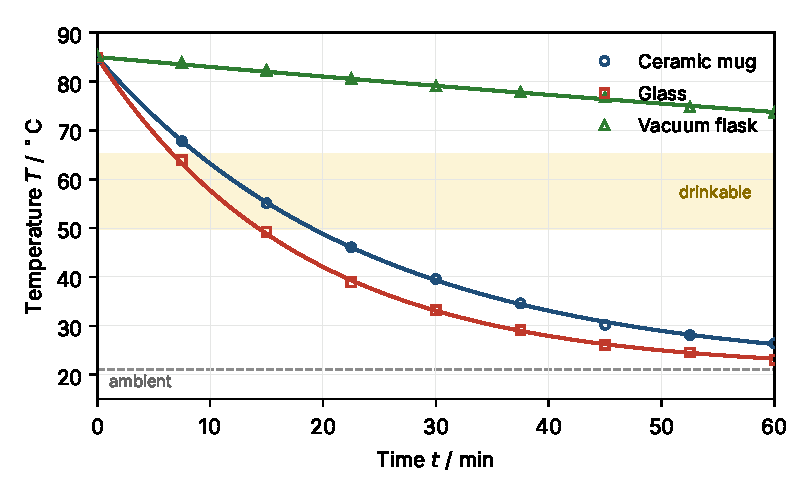
\includegraphics[width=0.8\textwidth]{figures/cooling-curves.pdf}
    \caption{Measured and modelled cooling curves.}
    \label{fig:cooling}
\end{figure}
>>>

% TODO 4.3: Cross-references
<<<
@0
%   Replace every number typed by hand with a reference.
%   1. Label each \section, on the same line:
%      \section{Theory}\label{sec:theory}
%   2. Label equations (1) and (2):
%      \begin{equation}\label{eq:cooling} and \label{eq:waiting}
%   3. Replace the typed numbers with Table~\ref{tab:vessels},
%      Figure~\ref{fig:cooling}, Section~\ref{sec:theory} and
%      Equation~\eqref{eq:cooling}.
%   Search for "TODO 4.3" to find all of them.
@4
>>>
% TODO 4.4: Clickable references
<<<
@0
%   1. Load hyperref (TODO 4.4 in the preamble).
%   2. Replace Table~\ref, Figure~\ref and Section~\ref with \autoref,
%      e.g. \autoref{fig:cooling}. Keep Equation~\eqref for equations.
%   Search for "TODO 4.4" to find all of them.
@4
>>>
<<<
@0
% Figure 1 shows the measured temperatures together with the model of Equation (1).
% All three vessels follow the exponential closely; what separates them is only the time constant listed in Table 1.
%
% Feeding those time constants into Equation (2) gives the drinkable window of Section 2 directly.
% The \texttt{mug} enters it about 9 minutes after pouring and leaves it after 19,
% which is the ten-minute window most people will recognise.
% The \texttt{glass} gives only seven minutes.
% The \texttt{flask} is still too hot to drink almost two hours later,
% which is either its great virtue or its great flaw,
% depending on what you wanted from it.
@4
\autoref{fig:cooling} shows the measured temperatures together with the model of Equation~\eqref{eq:cooling}.
All three vessels follow the exponential closely; what separates them is only the time constant listed in \autoref{tab:vessels}.

Feeding those time constants into Equation~\eqref{eq:waiting} gives the drinkable window of \autoref{sec:theory} directly.
The \texttt{mug} enters it about 9 minutes after pouring and leaves it after 19,
which is the ten-minute window most people will recognise.
The \texttt{glass} gives only seven minutes.
The \texttt{flask} is still too hot to drink almost two hours later,
which is either its great virtue or its great flaw,
depending on what you wanted from it.
>>>

% TODO 1.3: Sections
<<<
@0
%   \section{Conclusion} goes here.
@1
\section{Conclusion}
@4
\section{Conclusion}\label{sec:conclusion}
>>>

% TODO 4.2: Figure
<<<
@0
% Newton's law of cooling describes all three vessels well over a full hour,
% with a single time constant each.
% The practical answer is that an open mug of coffee is worth drinking between roughly 9 and 19 minutes after it is poured,
% and that insulation does not so much keep the drink pleasant as postpone the moment it becomes so.
@4
Newton's law of cooling describes all three vessels well over a full hour,
with a single time constant each.
The practical answer is that an open mug of coffee is worth drinking between roughly 9 and 19 minutes after it is poured,
and that insulation does not so much keep the drink pleasant as postpone the moment it becomes so.
>>>

% EXTRA (block 3, if you finish early): typesetting drills
%   These do not belong in the report.
%   Typeset them in display math here, look at the result, then delete them.
%   (a) The logistic map:
%       x_{t+1} = k x_t (1 - x_t)
%   (b) Shannon entropy:
%       H = - sum from i = 0 to N of p(x_i) log p(x_i)
%   (c) Hard mode, the inverse Laplace transform:
%       L^-1{F} = lim as T -> infinity of 1/(2 pi i) times the integral
%       from gamma - iT to gamma + iT of e^(st) F(s) ds

% TODO 4.5: Citation
<<<
@0
%   1. Load biblatex and add references.bib (TODO 4.5 in the preamble).
%   2. In the Theory section, replace the typed [1, 2] with
%      \parencite{halliday2018,incropera2007}.
%   3. Add \printbibliography here and compile.
@4
\printbibliography
>>>

% TODO 4.6: Broken citation, then fixed (optional)
%   Misspell one key in your \parencite, e.g. halliday2019, and compile.
%   Look at the PDF, then find the warning in the log.
%   Fix the key and compile again.

\end{document}
